\section{Efficiency and charge after a discharge}\label{app:recovery}
\tbw{Each reference-matched track is placed by the time since the last discharge on its chamber (a chip with ${\ge}8$ strips
over 3000\,ADC), and its detection efficiency and median charge are compared with tracks more than 1\,s after a
discharge (\cref{fig:sparkdt}). Neither moves at any delay we resolve; the integrated dead time per discharge is
fitted below 0.1\,s. The first bin (0--3\,ms) holds few tracks (53 on chamber~A), so this bounds the recovery but does
not measure it.}
\begin{figure}[t]
  \centering
  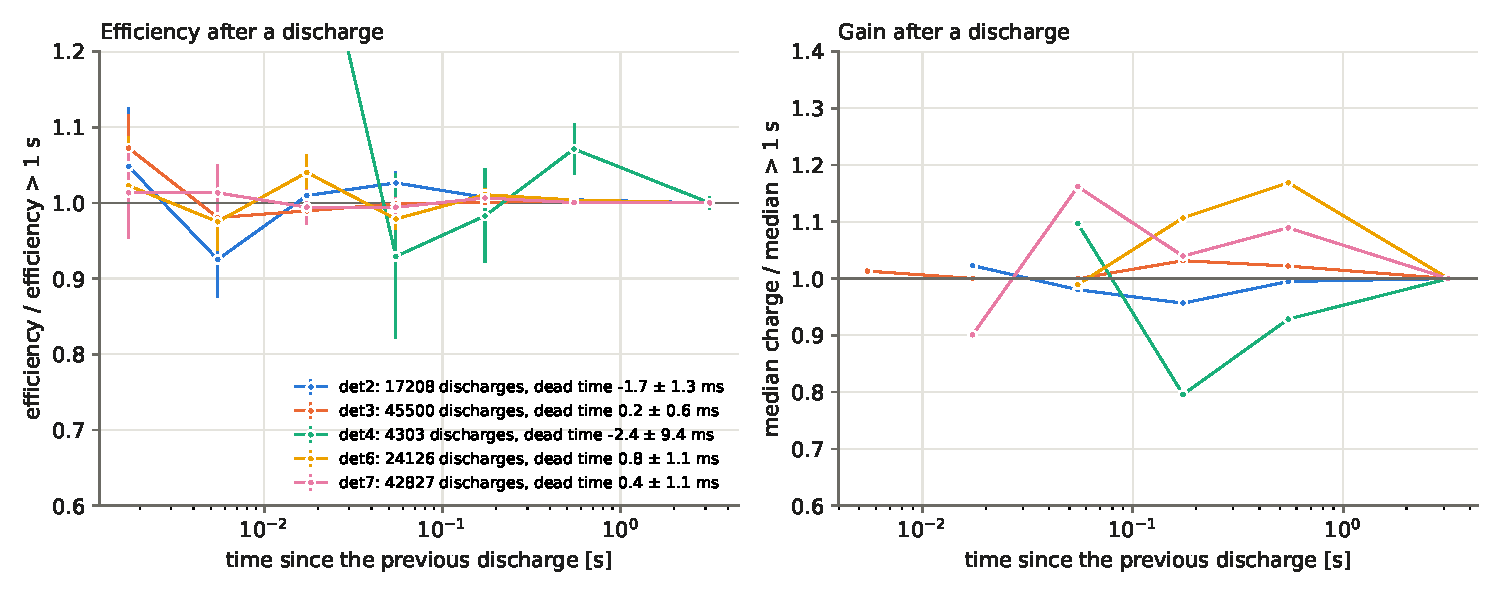
\includegraphics[width=\linewidth]{spark_deadtime}
  \caption{\tbw{(a) Detection efficiency and (b) median charge $Q_{50}$ against the time since the previous discharge, each relative to its value more than 1\,s after it; (c) chamber~E on its own scale. Discharges: A 45\,500, B 17\,208, C 24\,126, D 42\,827, E 4\,303. Charge errors from a bootstrap. Fitted dead time per discharge: A $0.2\pm0.6$, B $-1.7\pm1.3$, C $0.8\pm1.1$, D $0.4\pm1.1$, E $-2.4\pm9.4$\,ms: none.}}
  \label{fig:sparkdt}
\end{figure}
